\chapter{Testes da aplicação Nuxt}
\label{cap:nuxt-tests}
\minitoc

\intro{Como já mencionado, os testes da aplicação de front end não foram incluídos na monografia, pois estes não
haviam sido implementados até então.
Quase um mês depois da entrega, um bom avanço foi feito.
Este avanço é o objeto deste capítulo adicional}

\begin{figure}[ht]
    \centering
    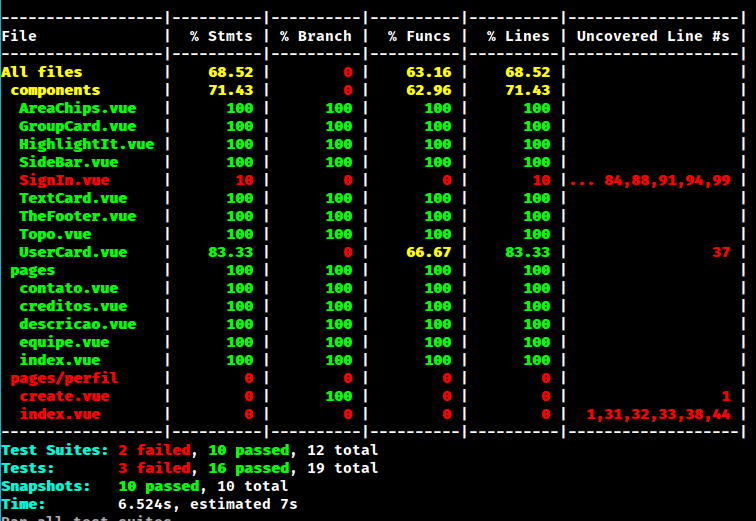
\includegraphics[width=.8\textwidth]{figuras/front-test.png}
    \caption{Resultado da execução de \texttt{yarn test}}
    \label{fig:test-nux}
\end{figure}

\section{Sobre as colunas}
\label{sec:colunas}

\begin{description}
    \item[Files] O nome do campo é auto explicativo
    \item[\% Stmts] Este campo retrata a fração de comandos (statements) que foram executados
    \item[\% Branch] Não é um teste sobre as versões (branches) do Github.
    A cada \texttt{if}, dois caminhos se abrem em uma determinada execução.
    Essa coluna atesta quantos desses \say{caminhos} foram verificados.
    \item[\% Funcs] Verifica a porcentagem de funções que foram chamadas
    \item[\% Lines] Verifica a porcentagem de linhas executáveis que foram chamadas.
    \item[Uncoverd Lines \#s] Também se trata de um campo auto explicativo
\end{description}

\section{Explicando os resultados}
\label{sec:results}

\begin{description}
    \item[Test Suit] Conjunto de testes agrupados em um arquivo
    \item[Snapshot] É como uma foto de um componente.
    É tirada na primeira execução de um teste que precisa dele, e não se altera a não ser que se inclua
    a flag \texttt{-u}\footnote{relativo a \texttt{--update-snapshot}} ao comando de teste.
    Quando o desenvolvedor remove ou altera o teste que pedia determinado Snapshot de modo que este se torne
    desnecessário, o programador pode removê-lo com a opção \texttt{-u} também
\end{description}

\paragraph{Testes com falha} Os testes que apresentaram problemas são aqueles que dependem de um determinado
módulo: Vuex.
Este permite que se crie métodos e variáveis disponíveis globalmente, coisa que não é possível de se fazer
só com os componentes.
A principal dificuldade é criar uma réplica do \say{store}\footnote{um módulo que contém as variáveis e os métodos}
e incluí-lo no componente para que este funcione da maneira correta.